\documentclass[border=6pt]{standalone}
\usepackage{lmodern}
\usepackage[T1]{fontenc}
\usepackage{amsmath}
\usepackage{xcolor}
\usepackage{tikz}
\usetikzlibrary{arrows.meta}
\definecolor{cblue}{HTML}{2F7DC8}
\definecolor{camber}{HTML}{E0891E}
\definecolor{cink}{HTML}{2B2B2B}
\tikzset{crv/.style={line width=0.9pt,smooth,samples=110}}
\newcommand{\gau}[2]{1.35*exp(0-((#1-#2)*(#1-#2))/2)}
\begin{document}
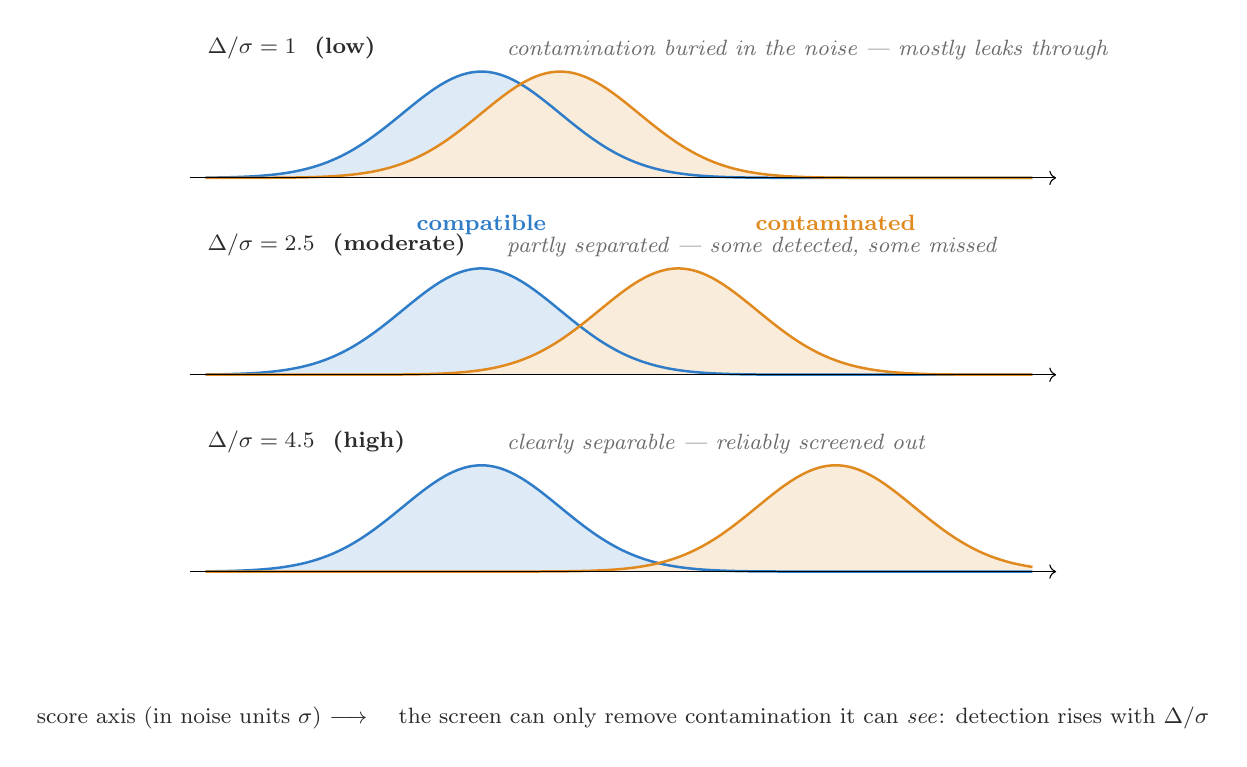
\begin{tikzpicture}[font=\small,x=1cm,y=1cm]
\foreach \row/\mu/\lab/\note in {%
   0/1.0/{$\Delta/\sigma=1$ \ (low)}/{contamination buried in the noise --- mostly leaks through},
   1/2.5/{$\Delta/\sigma=2.5$ \ (moderate)}/{partly separated --- some detected, some missed},
   2/4.5/{$\Delta/\sigma=4.5$ \ (high)}/{clearly separable --- reliably screened out}}{
  \begin{scope}[yshift={-\row*2.5cm}]
    \fill[cblue!16] (-3.5,0) -- plot[domain=-3.5:7,samples=90] (\x,{\gau{\x}{0}}) -- (7,0) -- cycle;
    \fill[camber!16] (-3.5,0) -- plot[domain=-3.5:7,samples=90] (\x,{\gau{\x}{\mu}}) -- (7,0) -- cycle;
    \draw[cblue,crv] plot[domain=-3.5:7] (\x,{\gau{\x}{0}});
    \draw[camber,crv] plot[domain=-3.5:7] (\x,{\gau{\x}{\mu}});
    \draw[->] (-3.7,0) -- (7.3,0);
    \node[anchor=west,font=\footnotesize\bfseries,text=cink] at (-3.6,1.65) {\lab};
    \node[anchor=west,font=\footnotesize\itshape,text=cink!70] at (0.2,1.62) {\note};
  \end{scope}
}
% shared legend
\node[cblue,font=\footnotesize\bfseries,anchor=north] at (0,-0.35) {compatible};
\node[camber,font=\footnotesize\bfseries,anchor=north] at (4.5,-0.35) {contaminated};
\node[anchor=north,font=\footnotesize,text=cink] at (1.8,-6.6)
  {score axis (in noise units $\sigma$) $\longrightarrow$ \quad the screen can only remove contamination it can \emph{see}: detection rises with $\Delta/\sigma$};
\end{tikzpicture}
\end{document}
